\documentclass{article}

% Language setting
% Replace `english' with e.g. `spanish' to change the document language
\usepackage[english]{babel}

% Set page size and margins
% Replace `letterpaper' with`a4paper' for UK/EU standard size
\usepackage[letterpaper,top=2cm,bottom=2cm,left=3cm,right=3cm,marginparwidth=1.75cm]{geometry}

% Useful packages
\usepackage{amsmath}
\usepackage{graphicx}
\usepackage[colorlinks=true, allcolors=blue]{hyperref}
\usepackage{tabularx}
\usepackage{fvextra}
\usepackage{ulem}

\title{Rapport d'avancement}
\author{Vital FOCHEUX}
\date{du 12 juin au 18 juin}

\begin{document}

\maketitle

\section{Notes de la dernière réunion}

\begin{itemize}
    \item Faire les spectres fréquentiels des signaux avant et après filtrage pour les analyser
    \item Refaire les tests des filtres passe-bas et passe-haut avec un $\tau$ différent pour chaque filtre
    \item Expliquer la génération du bruit pour le filtre médian, ainsi que revoir l'équation du signal généré
    \item Avoir les métriques du dépassement maximal et du temps de stabilisation pour les différents anti-windup
    \item Comprendre pourquoi les anti-windups passaient de 13 tour/min à 8 tour/min instantanément
\end{itemize}

\section{Planning}

\begin{itemize}
    \item \sout{du 8 au 12 juin :} 
    \begin{itemize}
        \item \sout{Correction du modèle de drone $\rightarrow$ pour qu'il fonctionne avec une consigne plus cohérente (5 mètres) et qu'on observe des résultats différents entre avec/sans anti-windup}
        \item \sout{Séparation filtres/contrôleurs}
        \item \sout{Clarifier l'interface chips $\rightarrow$ montrer comment utiliser Filtre/Anti-windup en chips avec description bloc fonctionnel et documentation}
        \item \sout{Plan détaillé du rapport de stage}
    \end{itemize}
    \item du 15 au 19 juin :
    \begin{itemize}
        \item Rédaction du package contrôleur chips (diagramme bloc fonctionnel + chips) $\rightarrow$ tester (via BIP)
        \item Des plots et diagrammes (pour analyser les résultats)
        \item Mise en commun avec Julien (travaux futurs)
    \end{itemize}
    \item du 22 au 26 juin :
    \begin{itemize}
        \item Rédaction du rapport de stage
        \item Lien formel travaux Vital / Motif control
    \end{itemize}
\end{itemize}

\section{Depuis la dernière fois}

\subsection{Filtre}

\subsubsection{Passe-bas et passe-haut}

Pour le filtre passe-bas et passe-haut, je me suis basé sur cet \href{https://www.geeksforgeeks.org/python/noise-removal-using-lowpass-digital-butterworth-filter-in-scipy-python/}{exemple}.
Mais le problème est que les signaux étaient trop proches l'un de l'autre, donc on ne voyait pas vraiment l'effet du filtre. 
Donc pour le filtre passe-bas et passe-haut, le signal est généré de la manière suivante :
$$y = \sin(2.0 * \pi * 10 * t) + \sin(2.0 * \pi * 200 * t)$$

Ce qui change c'est le $\tau$ du filtre, qui pour le filtre passe-bas est :
$$\tau = \frac{1}{2 * \pi * 50}$$ 
Pour garder les fréquences en dessous de 50 Hz.

Alors que pour le filtre passe-haut, le $\tau$ est :
$$\tau = \frac{1}{2 * \pi * 100}$$
Pour garder les fréquences au-dessus de 100 Hz.

Alors que pour l'exemple utilisant le filtre passe-haut puis passe-bas (cf. figure \ref{high_low_pass}), le signal est généré de la manière suivante :
$$y = \sin(2 * \pi * 5 * t) + \sin(2 * \pi * 100 * t) + \sin(2 * \pi * 400)$$

Et où le $\tau$ du filtre passe-haut est $\tau = \frac{1}{2 * \pi * 90}$ et le $\tau$ du filtre passe-bas est $\tau = \frac{1}{2 * \pi * 110}$

Pour chaque exemple on remarque avec le spectre fréquentiel (cf. figure \ref{fig:low_pass_fft}, \ref{fig:high_pass_fft} et \ref{high_low_pass_fft}) 
que les fréquences sont bien filtrées, et avec la densité spectrale de puissance (cf. figure \ref{fig:low_pass_psd}, \ref{fig:high_pass_psd} et \ref{high_low_pass_psd}) 
que le bruit est bien réduit. Le bruit est bien réduit mais tant que ça non plus, j'ai remarqué que la formule que j'utilise pour les filtres passe-bas et passe-haut 
sont celle qu'on peut retrouver sur \href{https://en.wikipedia.org/wiki/Low-pass_filter#Finite_impulse_response}{wikipedia pour passe-bas} et \href{https://en.wikipedia.org/wiki/High-pass_filter}{wikipedia pour passe-haut} 
sauf qu'elles sont d'ordre de précision 1, donc ça ne filtre pas beaucoup. Il faudrait que je fasse un filtre d'ordre 2 ou plus pour que le bruit soit encore plus réduit.
En faisant, des recherches je suis tombé sur Runge-Kutta 4 (RK4) qui est un algorithme d'ordre 4, donc je vais essayer de l'implémenter pour voir si le bruit est encore plus réduit.

\begin{figure}
    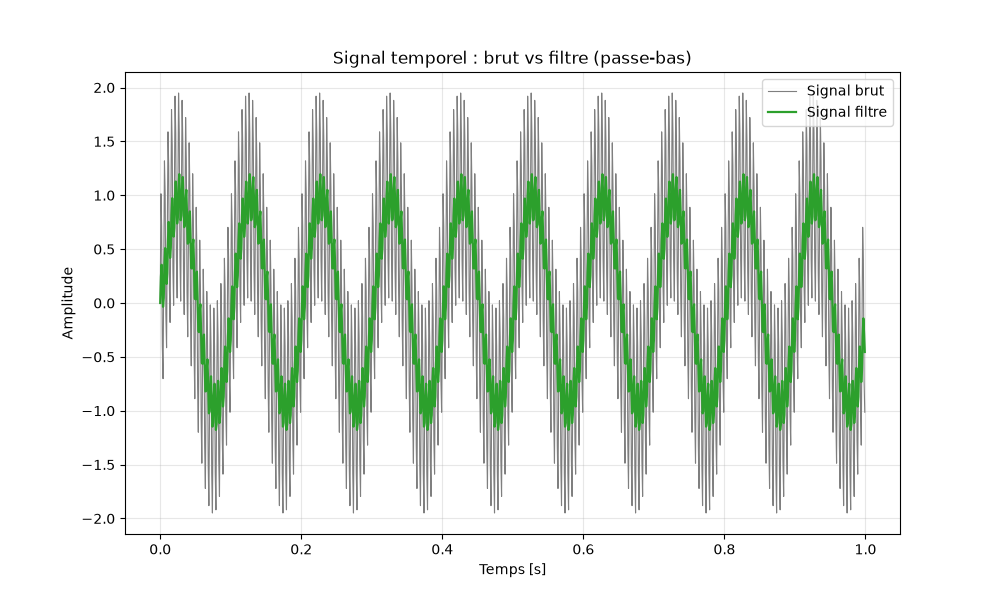
\includegraphics[width=\textwidth]{low_pass.png}
    \caption{Résultat du filtre passe-bas sur des fréquences avec du bruit}
    \label{fig:low_pass}
\end{figure}

\begin{figure}
    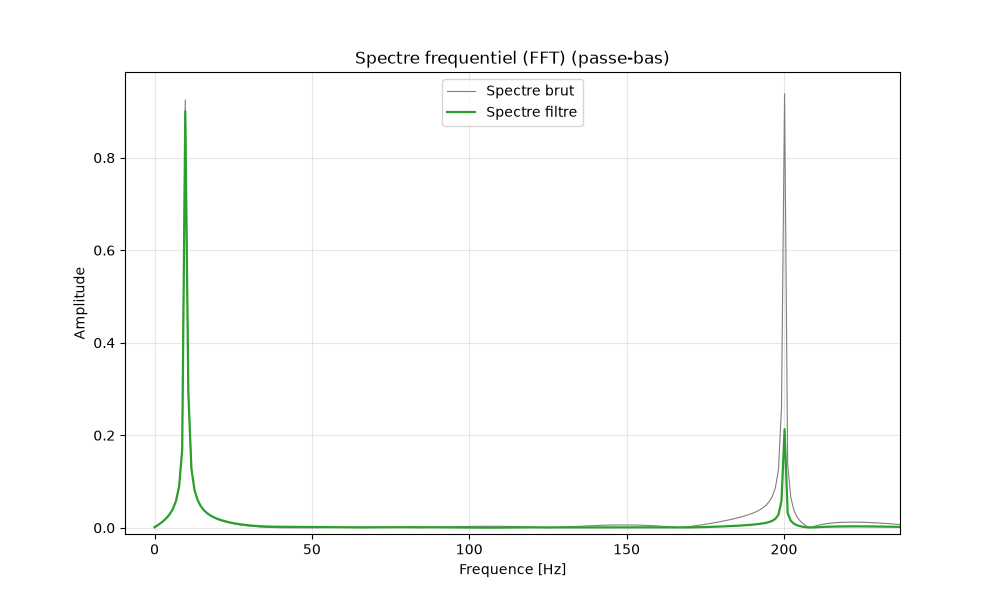
\includegraphics[width=\textwidth]{low_pass_fft.png}
    \caption{Spectre fréquentiel du signal avant et après le filtre passe-bas}
    \label{fig:low_pass_fft}
\end{figure}

\begin{figure}
    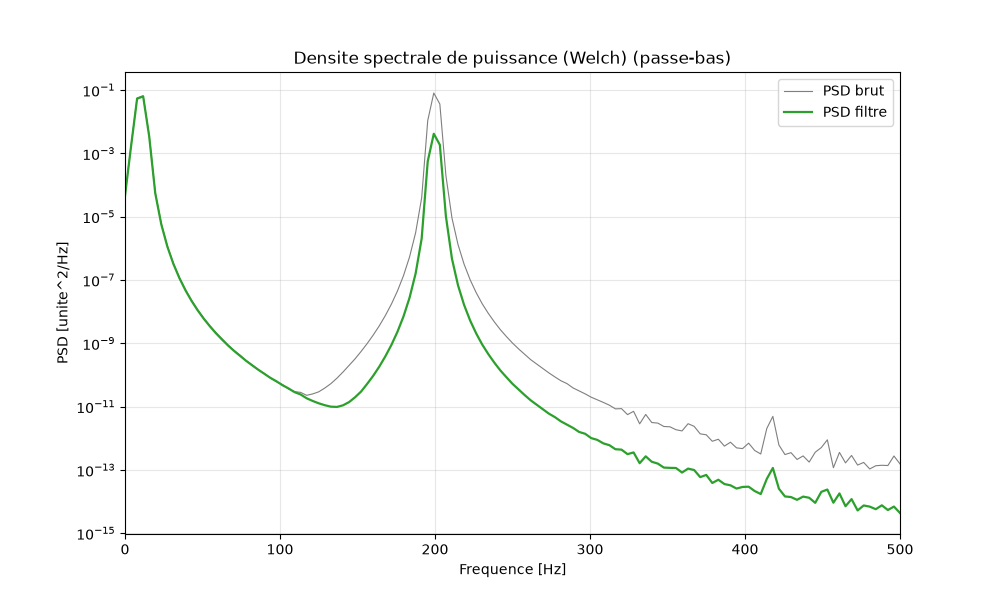
\includegraphics[width=\textwidth]{low_pass_psd.png}
    \caption{Densité spectrale de puissance du signal avant et après le filtre passe-bas}
    \label{fig:low_pass_psd}
\end{figure}

\begin{figure}
    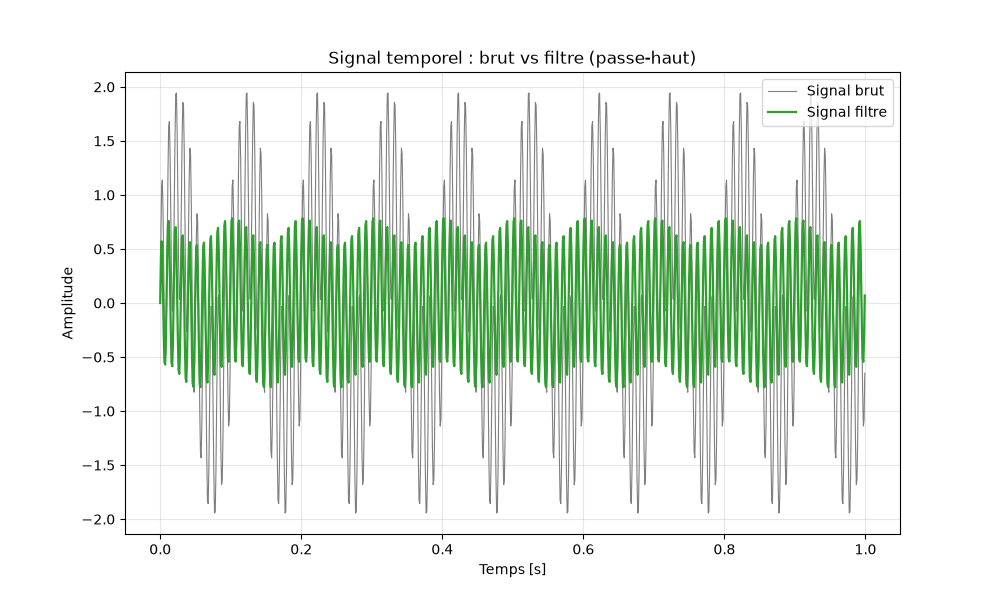
\includegraphics[width=\textwidth]{high_pass.png}
    \caption{Résultat du filtre passe-haut sur les fréquences avec du bruit}
    \label{fig:high_pass}
\end{figure}

\begin{figure}
    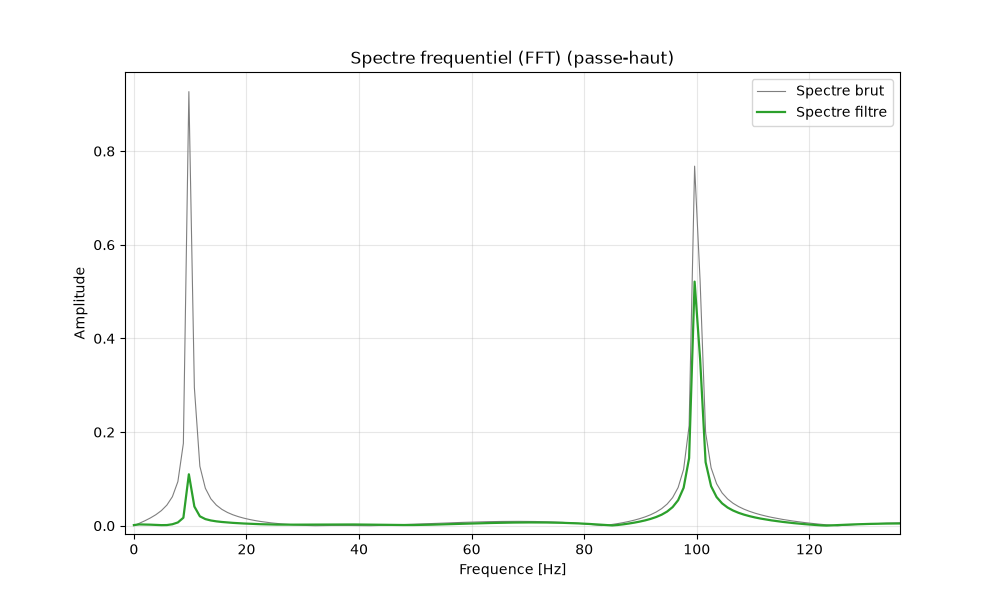
\includegraphics[width=\textwidth]{high_pass_fft.png}
    \caption{Spectre fréquentiel du signal avant et après le filtre passe-haut}
    \label{fig:high_pass_fft}
\end{figure}

\begin{figure}
    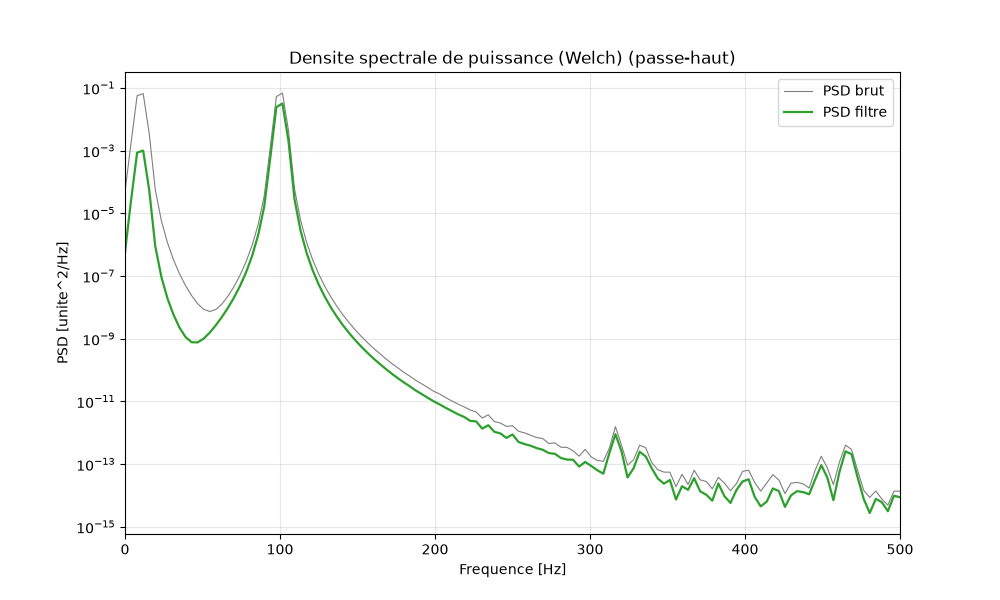
\includegraphics[width=\textwidth]{high_pass_psd.png}
    \caption{Densité spectrale de puissance du signal avant et après le filtre passe-haut}
    \label{fig:high_pass_psd}
\end{figure}

\begin{figure}
    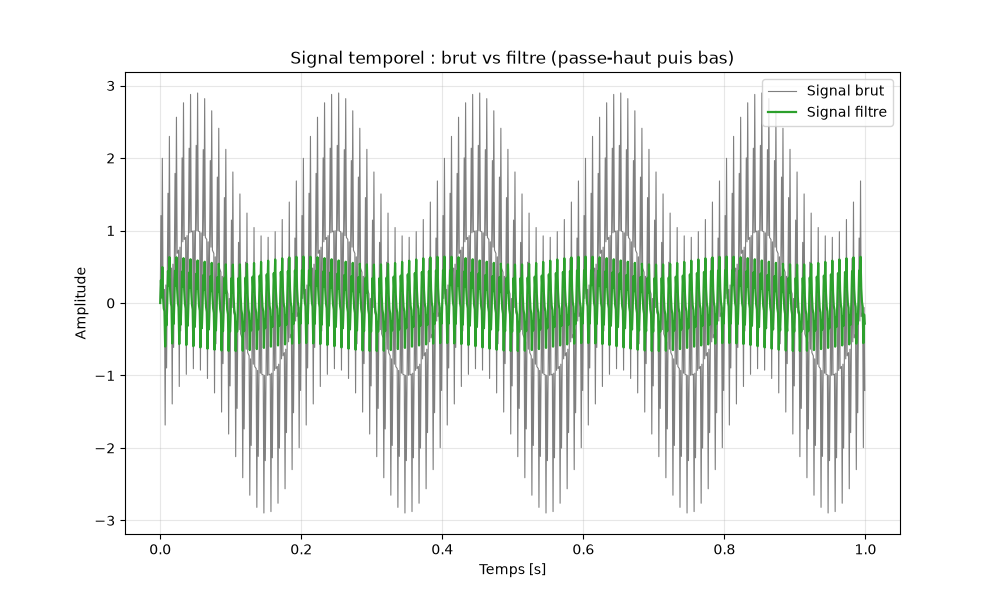
\includegraphics[width=\textwidth]{high_low_pass.png}
    \caption{Résultat du filtre passe-haut puis basse-bas sur les fréquences avec du bruit}
    \label{high_low_pass}
\end{figure}

\begin{figure}
    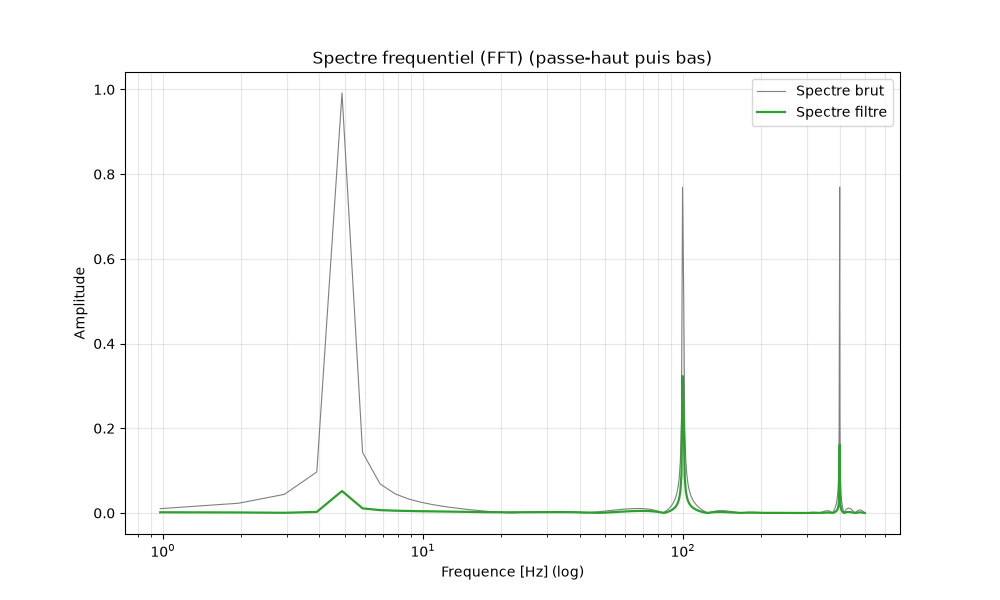
\includegraphics[width=\textwidth]{high_low_fft.png}
    \caption{Spectre fréquentiel du signal avant et après le filtre passe-haut puis basse-bas}
    \label{high_low_pass_fft}
\end{figure}

\begin{figure}
    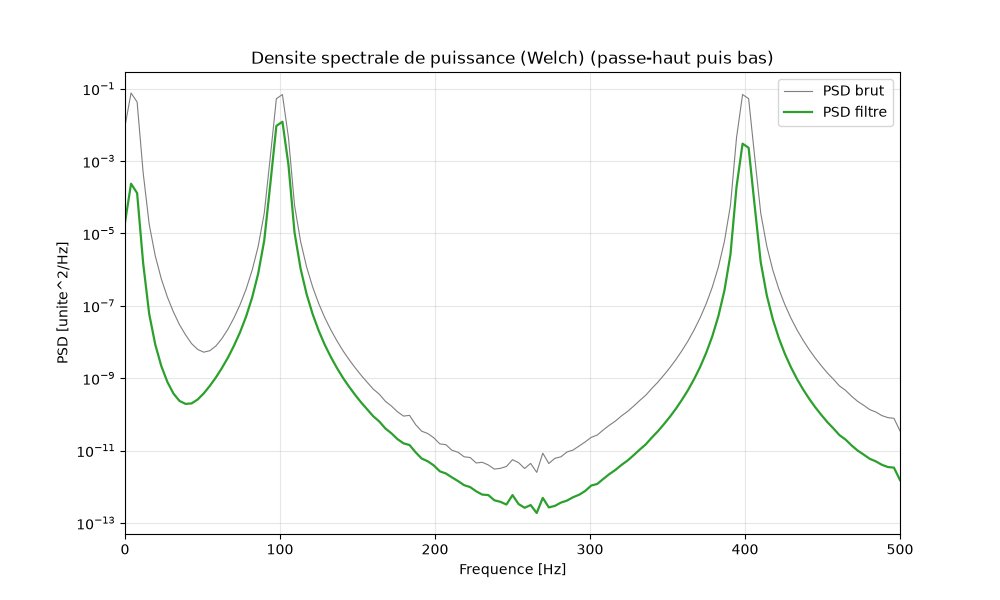
\includegraphics[width=\textwidth]{high_low_pass_psd.png}
    \caption{Densité spectrale de puissance du signal avant et après le filtre passe-haut puis basse-bas}
    \label{high_low_pass_psd}
\end{figure}

\subsubsection{Median}

Les données sont générées de tel manière :
$$y = sin(2.0 * \pi * freq * time) + spike $$

Où :
\begin{itemize}
    \item $freq$ est la fréquence du signal, ici 0.2
    \item $time$ est le temps, ici de 0 à 10 secondes avec un pas de 0.05 secondes
    \item $spike$ est un pic qui est égal à 2 toutes les 2 secondes, et 0 sinon
\end{itemize}

On peut remarquer que si on applique le filtre avec une fenêtre de 5, on obtient un signal qui est très proche du 
signal d'origine, mais avec moins de bruit. (cf. figure \ref{fig:median})
Cependant si on augmente la taille de la fenêtre à 10 ou 15, on obtient un signal décalé dans le temps et qui est moins précis. (cf. figure \ref{fig:median_10} et \ref{fig:median_15})


\begin{figure}
    
\includegraphics[width=\textwidth]{median.png}
    \caption{Résultat du filtre médian sur des fréquence avec des pics de bruit}
    \label{fig:median}
\end{figure}

\begin{figure}
    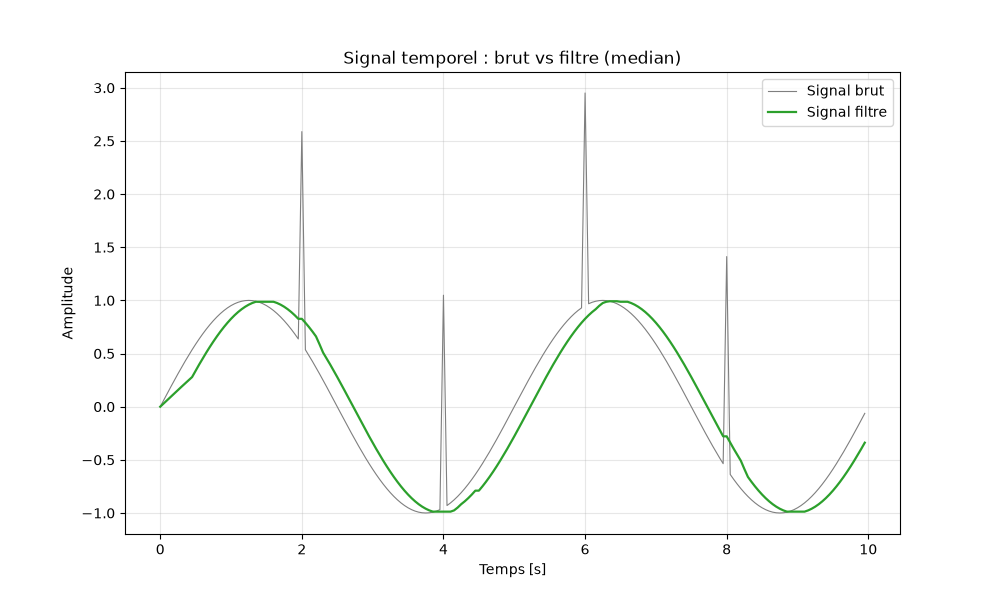
\includegraphics[width=\textwidth]{median_10.png}
    \caption{Résultat du filtre médian sur des fréquence avec des pics de bruit, avec une fenêtre de 10}
    \label{fig:median_10}
\end{figure}

\begin{figure}
    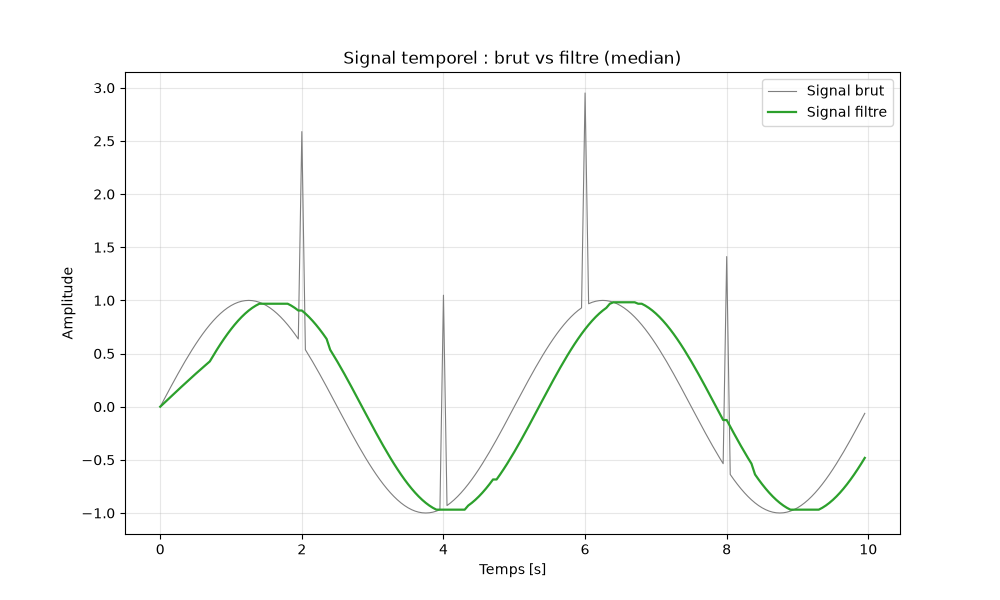
\includegraphics[width=\textwidth]{median_15.png}
    \caption{Résultat du filtre médian sur des fréquence avec des pics de bruit, avec une fenêtre de 15}
    \label{fig:median_15}
\end{figure}

\subsection{Anti-windup}

\subsubsection{Explication des pics à temps 0}

Le pic est dû au calcul de la dérivé car on fait $\frac{error - error_{prev}}{dt}$. Cette valeur est égal à 5 à temps 0 car il n'y a pas de valeur précédente, donc on prend la valeur actuelle qui est 5. 
Puis au temps suivant cette valeur est de 0 car l'erreur est de 5 et l'erreur précédente est de 5, donc la dérivé est de 0. Donc le pic est dû à la dérivé qui est calculée à temps 0.

\subsubsection{Métriques}

Les métriques du dépassement maximal et du temps de stabilisation pour les différents anti-windup sont les suivantes  et visibles sur la figure \ref{fig:anti_windup_altitude}, \ref{fig:anti_windup_integral} et \ref{fig:anti_windup_blade} :

\begin{tabular}{|c|c|c|}
    \hline & Dépassement maximal (m) & Temps de stabilisation ($\pm 5\%$) (s) \\    
    \hline Sans anti-windup & 12.00 & 32.2\\
    \hline Anti-windup clamp & 7.32 & 21.6\\
    \hline Anti-windup back-calculation & 5.31 & 18.9\\
    \hline
\end{tabular}

\begin{tabular}{|c|c|c|}
    \hline & Intégrale maximale & Commande moyenne (tour/min) \\
    \hline Sans anti-windup & 60.86 & 12.78\\
    \hline Anti-windup clamp & 30 & 12.86\\
    \hline Anti-windup back-calculation & 21.9 & 12.88 \\
    \hline    
\end{tabular}

\begin{figure}
    
\includegraphics[width=\textwidth]{anti_windup_altitude.png}
    \caption{Altitude drone avec différents anti-windup}
    \label{fig:anti_windup_altitude}
\end{figure}

\begin{figure}
    
\includegraphics[width=\textwidth]{anti_windup_integral.png}
    \caption{Intégrale des différents anti-windup}
    \label{fig:anti_windup_integral}
\end{figure}

\begin{figure}
    
\includegraphics[width=\textwidth]{anti_windup_blade.png}
    \caption{Vitesse de rotation des hélices avec différents anti-windup}
    \label{fig:anti_windup_blade}
\end{figure}

\section{Package}

Etant donné que le compilateur n'est pas encore fini. Je n'ai pas encore pu rédiger les packages chips, ainsi que les tester.

\end{document}